\documentclass[a4paper,10pt]{report}
\usepackage[utf8]{inputenc}
\usepackage{hyperref}
\usepackage{graphicx}

% Title Page
\title{Analyse de Comportements avec Twitter}
\author{Antonin Durey Matthieu Caron}




\begin{document}
\pagenumbering{alph}
\maketitle
\clearpage
\pagenumbering{arabic}
\chapter{Description générale du projet}
  \section{Lien vers le git}
    \url{https://github.com/Grimnack/pje2}
  \section{Description de la problématique}
    L'idée c'est de créer une application permettant de tester différents algorithmes
    afin de faire une analyse de sentiments sur twitter. La problématique est donc la suivante,
    quel est l'algorithme le plus efficace (qui donne le plus souvent la vérité) pour faire de la 
    classification de sentiments?
  \section{Architecture de l'application}
    Nous avons fait une application java swing. On utilise donc une architecture MVC, le controlleur étant 
    essentiellement 
\chapter{Détails des différents travaux réalisés}
  Le projet se divise en quatre taches majeures, utilisation de une API twitter afin de récupérer 
  des tweets, préparer une base d'apprentissage afin de ne pas avoir de bruit mais aussi de créer notre 
  base de vérité pour l'apprentissage supervisé. Implémenter et tester différents algorithmes de classification de sentiments et
  enfin pouvoir utiliser ses algorithme depuis une application avec son interface graphique.
  \section{API Twitter}
  % image de l'interface graphique et explication
  \section{Préparation de la base d'apprentissage}
    \subsection{Nettoyage des données}
      Pour nettoyer nos données :
      \begin{itemize}
       \item Pour les doublons, nous n'avons pas compté les retweets car un retweet c est donner un avis à nouveau.
       \item Nous avons retiré les tweets qui comportent des smileys positifs et négatifs en même temps.
       \item Nous avons fait un filtrage pour retirer  (enlever les @,  \#,  RT,  URL  et  l’URL  associé)
      \end{itemize}

    \subsection{Construction de la base}
      Pour construire notre base de tweets, nous le faisons directemment depuis notre application, nous récupèrons des tweets par 
      paquet de dix, et on peut cliquer sur \emph{Etiquettage} et ça permet de pouvoir ettiqueter chaque tweet en lui donnant la classe positive, negative ou neutre,
      pour ensuite ajouter ces tweets à notre base d'apprentissage grace a une selection de fichier.
      % image de l'interface
  \section{Algorithme de classification}
    Pour tester les différents algorithmes nous avons d'une part regardé si il y a une forte différence entre ce que trouve un humain et ce que trouve l'algorithme, d'autre part
    regardé le temps de calcul, lorsqu'on travaille sur les bigdata ce n'est pas négligeable.
    Pour 
    \subsection{mots clefs}
      Pour l'algorithme des mots clefs nous avons gardé le dictionnaire de mots intact, on a juste retiré ``communiste'' de la liste de mots négatifs.
      Pour ce qui est de l'efficacité en terme de réponses (si le jugement positif, negatif ou neutre est correcte) : on a 64\% de réponses correctes.
      Pour ce qui est du temps de calcul %%TODO chercher la valeur de la complexité
      
      
    \subsection{KNN}
      
    \subsection{Bayes}
  \section{Interface graphique}
    \subsection{copie d'ecran}
      \begin{figure}[!h]
	\centering
	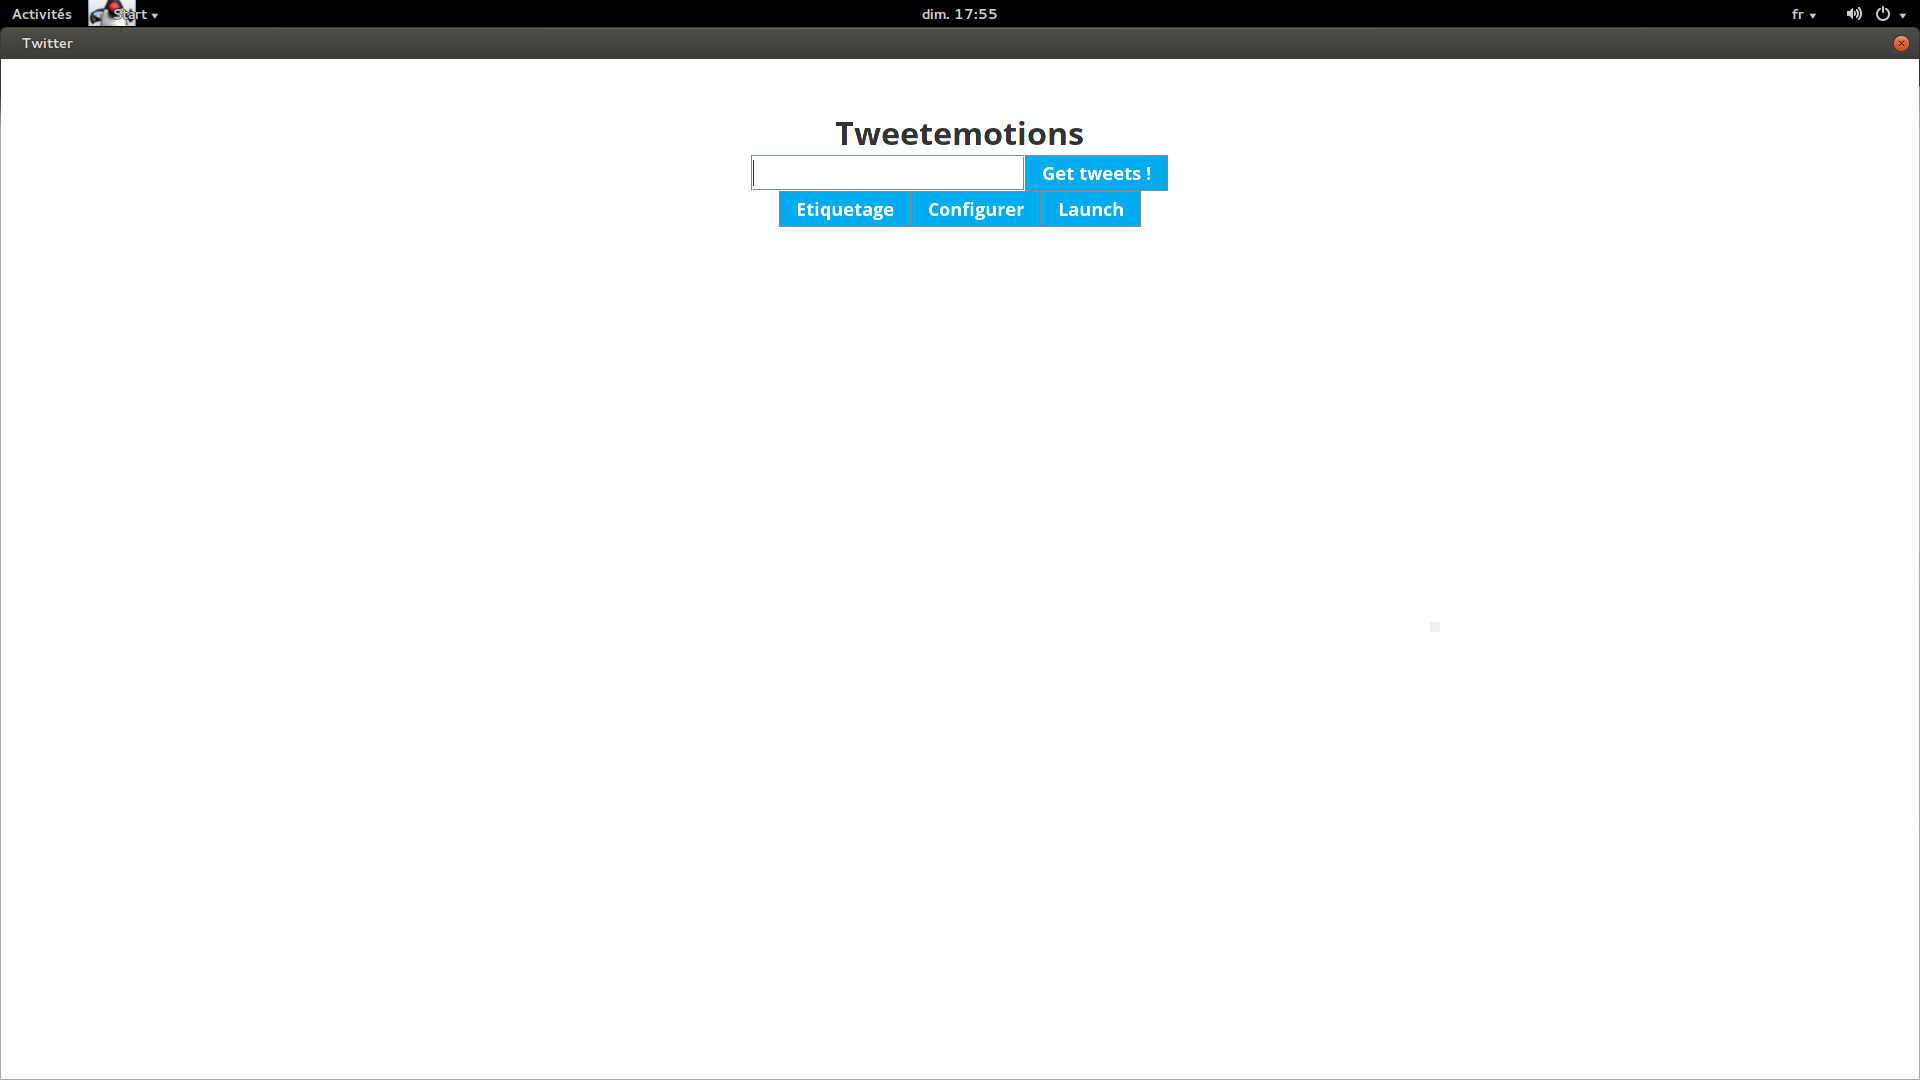
\includegraphics[scale=0.2]{impressions-ecran/accueil.png}
	\caption{Page d'accueil}
	\label{accueil}
      \end{figure}
      \begin{figure}[!h]
	\centering
	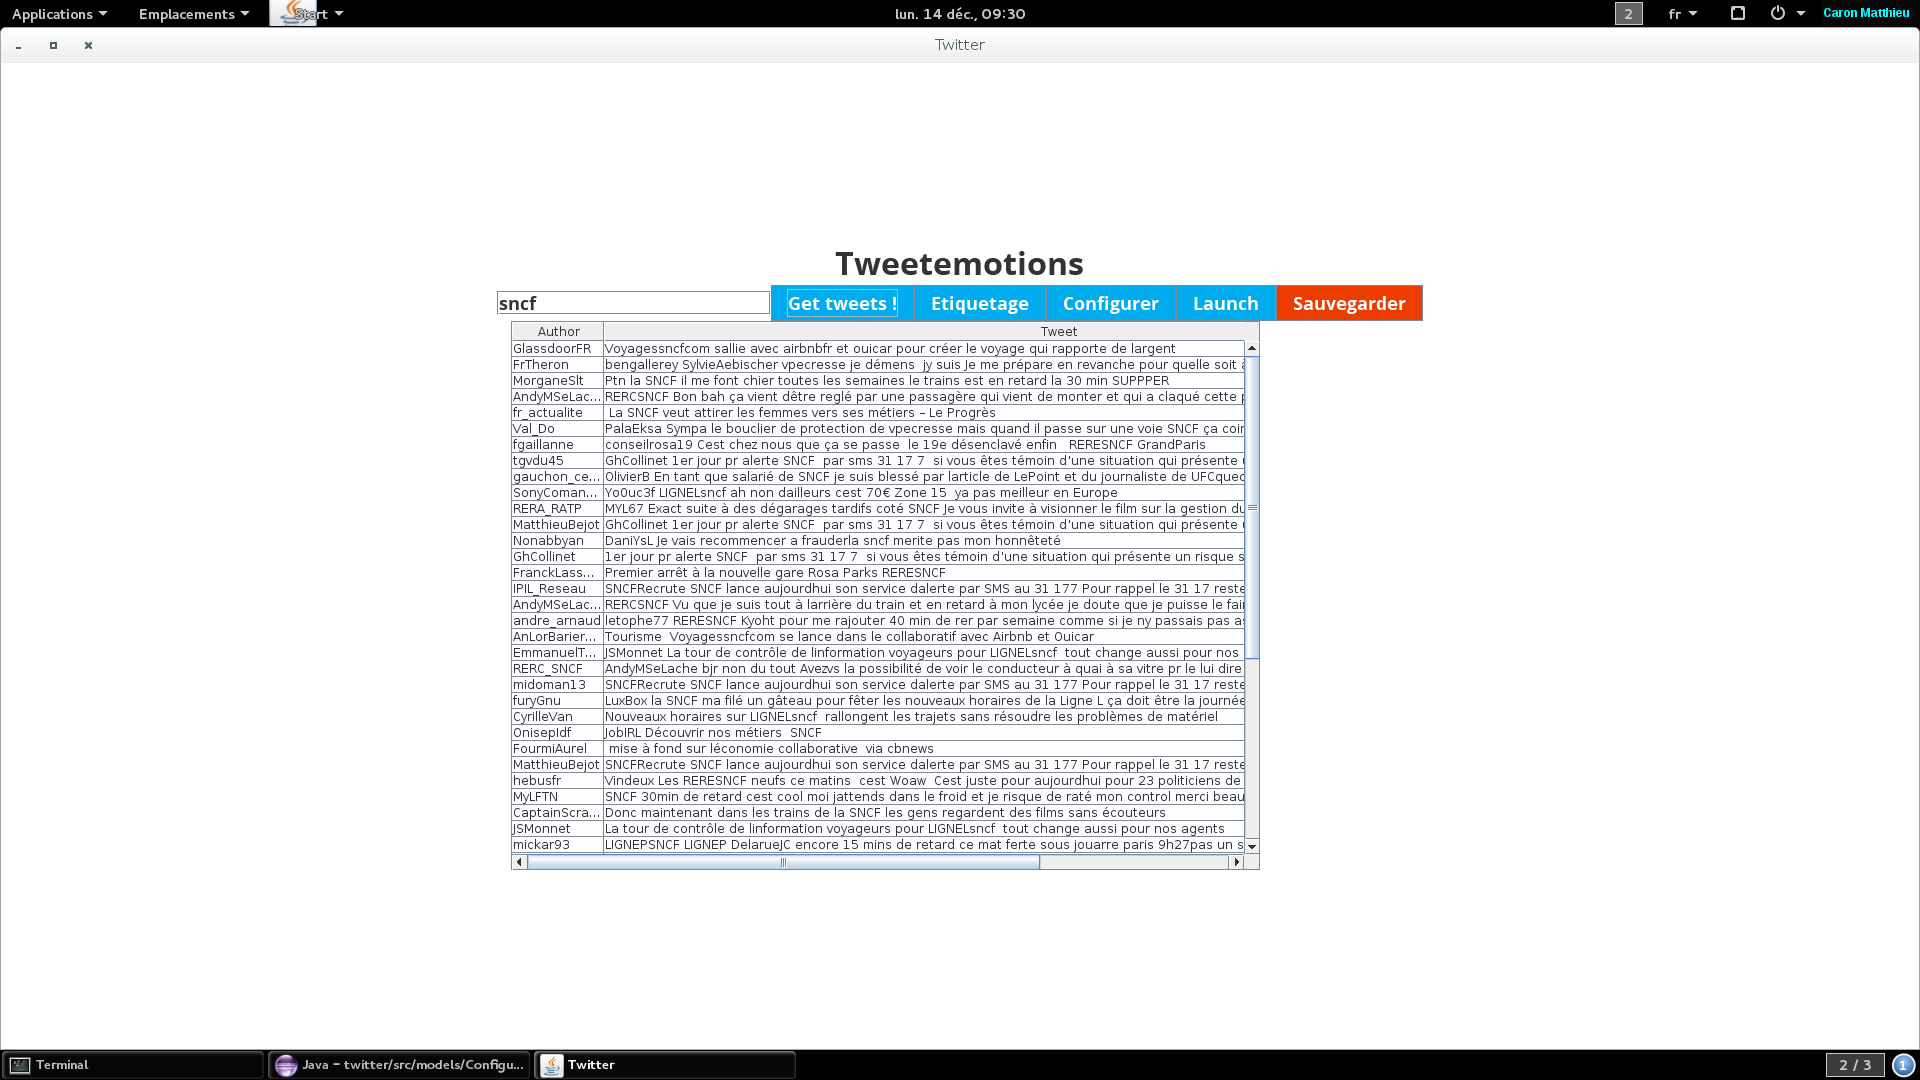
\includegraphics[scale=0.2]{impressions-ecran/tweets.png}
	\caption{Affichage des tweets}
	\label{tweets}
      \end{figure}
      \begin{figure}[!h]
	\centering
	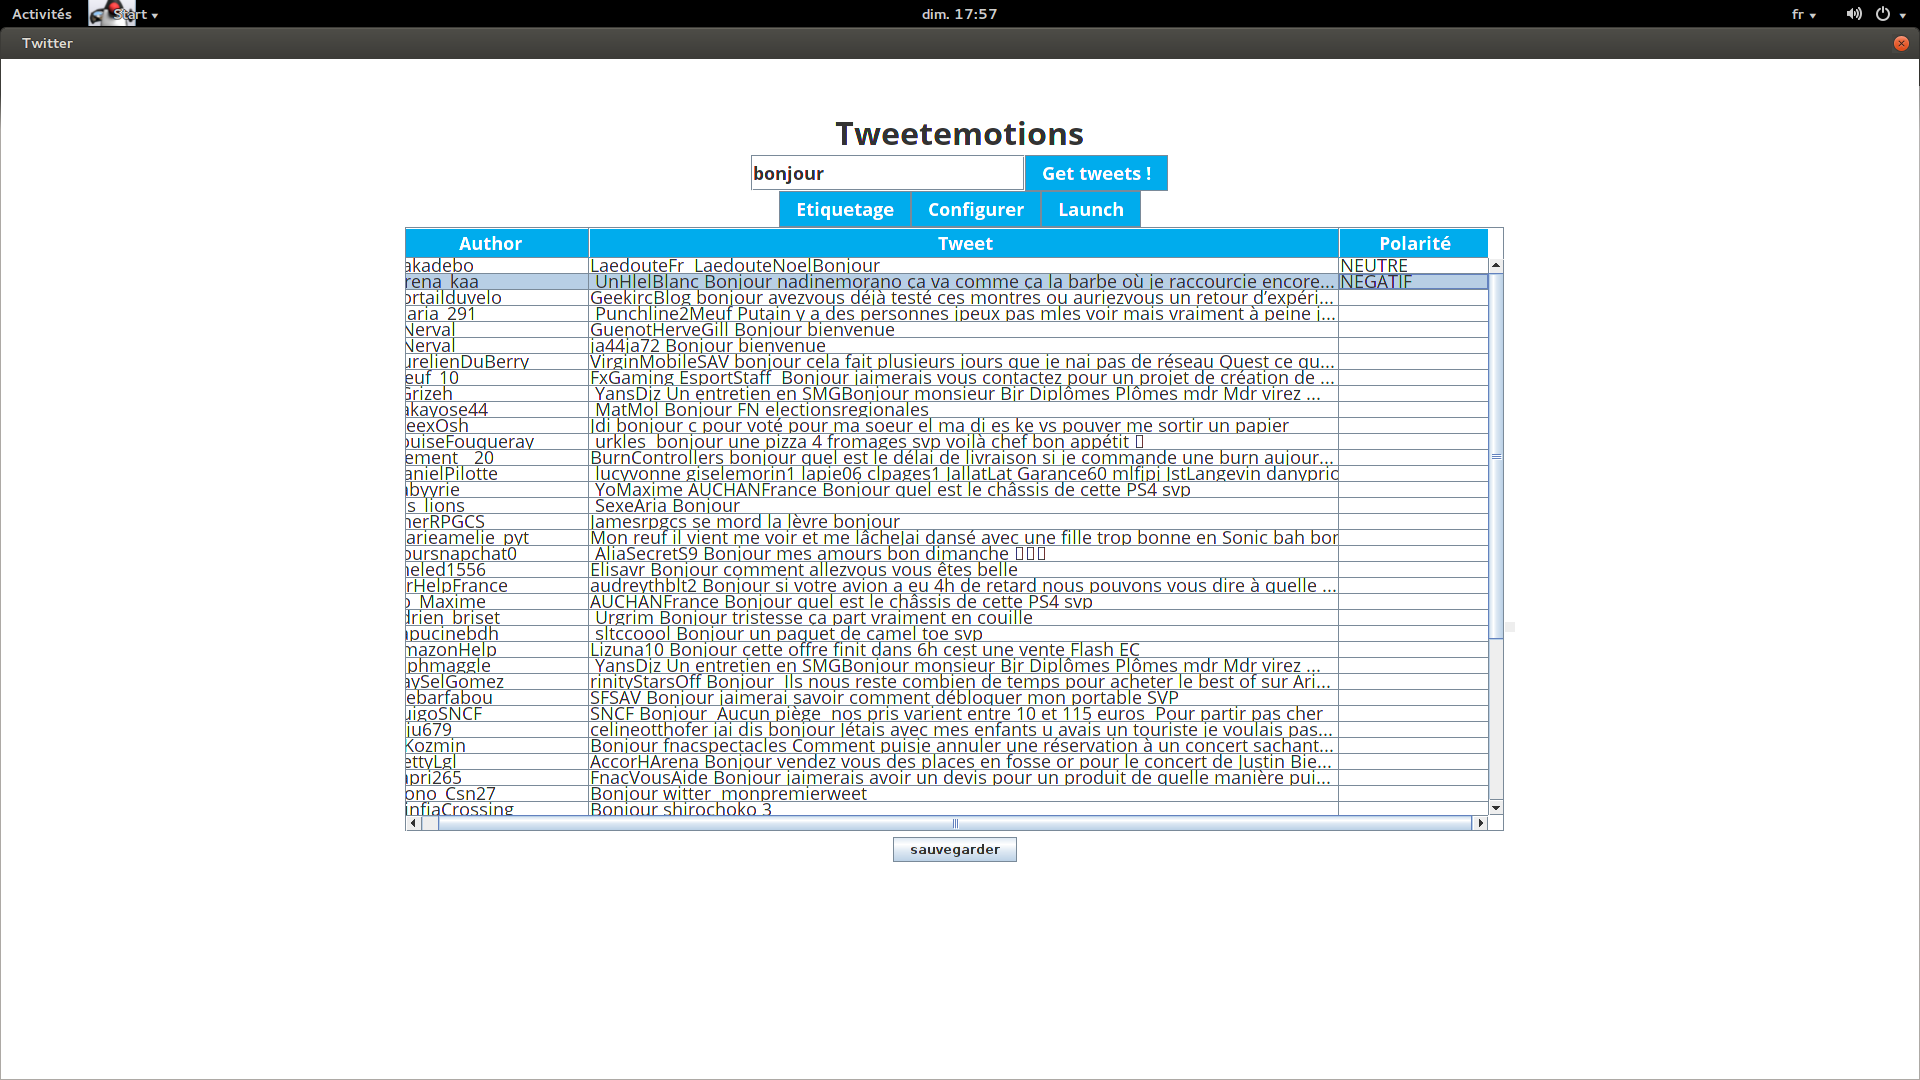
\includegraphics[scale=0.2]{impressions-ecran/etiquetage.png}
	\caption{Étiquetage des tweets}
	\label{etiquetage}
      \end{figure}



    
    \subsection{manuel d'utilisation}
      On lance l'application, la fenetre principale est composée d'un champ de texte, un bouton ``get tweets'', un bouton ``Etiquettage'', un bonton ``Configurer'' et 
      un bouton ``Launch''.
      \subsubsection{Le bouton ``Get Tweets''}
	Si vous cliquez sur le bouton ``Get Tweets'', l'application va vous demander combien de tweets vous souhaitez récupérer. Une fois le nombre de tweet choisit,
	il va chercher les tweets contenant la chaine de caractère écrite au préalable dans le champ de texte et va afficher ces tweets à l'écran.
	À partir de ce moment tous les calculs (dico, knn et bayes) se feront sur ces tweets.
      \subsubsection{Le bouton ``Etiquetage''}
	Ce bouton est utile pour ajouter des tweets à une base de données, il faut avoir au préalable cherché des tweets avec le bouton ``Get Tweets''.
	A côté de chaque tweet vous allez devoir choisir qu'elle est leur polarité, neutre, positif ou négatif. Une fois ceci fait pour tous les tweets, vous 
	allez pouvoir sauvegarder vos tweets étiquetés. Pour la sauvegarde un selecteur de fichiers s'ouvre, si vous choisissez un fichier de type .base existant
	les tweets annotés vont être ajouté a la base de tweets choisit. Vous pouvez aussi créer une nouvelle base, il est préférable de choisir l'extension .base
	pour se retrouver dans ses fichiers.
      \subsubsection{Le bouton ``Configurer''}
	Ce bouton sert a choisir l'algorithme de classification entre Dico, KNN et Bayes. 
\chapter{Résultats de la classification avec les différentes méthodes et analyse}
\chapter{Conclusions}




\end{document}     
